%!TeX encoding = UTF-8
%!TeX program = xelatex
\documentclass[notheorems, aspectratio=54]{beamer}
% aspectratio: 1610, 149, 54, 43(default), 32

\usepackage{latexsym}
\usepackage{amsmath,amssymb}
\usepackage{mathtools}
\usepackage{color,xcolor}
\usepackage{graphicx}
\usepackage{algorithm}
\usepackage{amsthm}
\usepackage{lmodern} % 解决 font warning
% \usepackage[UTF8]{ctex}
\usepackage{animate} % insert gif

\usepackage{lipsum} % To generate test text 
\usepackage{ulem} % 下划线,波浪线

\usepackage{listings} % display code on slides; don't forget [fragile] option after \begin{frame}

% ----------------------------------------------
% tikx
\usepackage{framed}
\usepackage{tikz}
\usepackage{pgf}
\usetikzlibrary{calc,trees,positioning,arrows,chains,shapes.geometric,%
    decorations.pathreplacing,decorations.pathmorphing,shapes,%
    matrix,shapes.symbols}
\pgfmathsetseed{1} % To have predictable results
% Define a background layer, in which the parchment shape is drawn
\pgfdeclarelayer{background}
\pgfsetlayers{background,main}

% define styles for the normal border and the torn border
\tikzset{
  normal border/.style={orange!30!black!10, decorate, 
     decoration={random steps, segment length=2.5cm, amplitude=.7mm}},
  torn border/.style={orange!30!black!5, decorate, 
     decoration={random steps, segment length=.5cm, amplitude=1.7mm}}}

% Macro to draw the shape behind the text, when it fits completly in the
% page
\def\parchmentframe#1{
\tikz{
  \node[inner sep=2em] (A) {#1};  % Draw the text of the node
  \begin{pgfonlayer}{background}  % Draw the shape behind
  \fill[normal border] 
        (A.south east) -- (A.south west) -- 
        (A.north west) -- (A.north east) -- cycle;
  \end{pgfonlayer}}}

% Macro to draw the shape, when the text will continue in next page
\def\parchmentframetop#1{
\tikz{
  \node[inner sep=2em] (A) {#1};    % Draw the text of the node
  \begin{pgfonlayer}{background}    
  \fill[normal border]              % Draw the ``complete shape'' behind
        (A.south east) -- (A.south west) -- 
        (A.north west) -- (A.north east) -- cycle;
  \fill[torn border]                % Add the torn lower border
        ($(A.south east)-(0,.2)$) -- ($(A.south west)-(0,.2)$) -- 
        ($(A.south west)+(0,.2)$) -- ($(A.south east)+(0,.2)$) -- cycle;
  \end{pgfonlayer}}}

% Macro to draw the shape, when the text continues from previous page
\def\parchmentframebottom#1{
\tikz{
  \node[inner sep=2em] (A) {#1};   % Draw the text of the node
  \begin{pgfonlayer}{background}   
  \fill[normal border]             % Draw the ``complete shape'' behind
        (A.south east) -- (A.south west) -- 
        (A.north west) -- (A.north east) -- cycle;
  \fill[torn border]               % Add the torn upper border
        ($(A.north east)-(0,.2)$) -- ($(A.north west)-(0,.2)$) -- 
        ($(A.north west)+(0,.2)$) -- ($(A.north east)+(0,.2)$) -- cycle;
  \end{pgfonlayer}}}

% Macro to draw the shape, when both the text continues from previous page
% and it will continue in next page
\def\parchmentframemiddle#1{
\tikz{
  \node[inner sep=2em] (A) {#1};   % Draw the text of the node
  \begin{pgfonlayer}{background}   
  \fill[normal border]             % Draw the ``complete shape'' behind
        (A.south east) -- (A.south west) -- 
        (A.north west) -- (A.north east) -- cycle;
  \fill[torn border]               % Add the torn lower border
        ($(A.south east)-(0,.2)$) -- ($(A.south west)-(0,.2)$) -- 
        ($(A.south west)+(0,.2)$) -- ($(A.south east)+(0,.2)$) -- cycle;
  \fill[torn border]               % Add the torn upper border
        ($(A.north east)-(0,.2)$) -- ($(A.north west)-(0,.2)$) -- 
        ($(A.north west)+(0,.2)$) -- ($(A.north east)+(0,.2)$) -- cycle;
  \end{pgfonlayer}}}

% Define the environment which puts the frame
% In this case, the environment also accepts an argument with an optional
% title (which defaults to ``Example'', which is typeset in a box overlaid
% on the top border
\newenvironment{parchment}[1][Example]{%
  \def\FrameCommand{\parchmentframe}%
  \def\FirstFrameCommand{\parchmentframetop}%
  \def\LastFrameCommand{\parchmentframebottom}%
  \def\MidFrameCommand{\parchmentframemiddle}%
  \vskip\baselineskip
  \MakeFramed {\FrameRestore}
  \noindent\tikz\node[inner sep=1ex, draw=black!20,fill=white, 
          anchor=west, overlay] at (0em, 2em) {\sffamily#1};\par}%
{\endMakeFramed}

% ----------------------------------------------

\mode<presentation>{
    \usetheme{CambridgeUS}
    % Boadilla CambridgeUS
    % default Antibes Berlin Copenhagen
    % Madrid Montpelier Ilmenau Malmoe
    % Berkeley Singapore Warsaw
    \usecolortheme{beaver}
    % beetle, beaver, orchid, whale, dolphin
    \useoutertheme{infolines}
    % infolines miniframes shadow sidebar smoothbars smoothtree split tree
    \useinnertheme{circles}
    % circles, rectanges, rounded, inmargin
}
% 设置 block 颜色
\setbeamercolor{block title}{bg=red!30,fg=white}

\newcommand{\reditem}[1]{\setbeamercolor{item}{fg=red}\item #1}

% 缩放公式大小
\newcommand*{\Scale}[2][4]{\scalebox{#1}{\ensuremath{#2}}}

% 解决 font warning
\renewcommand\textbullet{\ensuremath{\bullet}}

% ---------------------------------------------------------------------
% flow chart
\tikzset{
    >=stealth',
    punktchain/.style={
        rectangle, 
        rounded corners, 
        % fill=black!10,
        draw=white, very thick,
        text width=6em,
        minimum height=2em, 
        text centered, 
        on chain
    },
    largepunktchain/.style={
        rectangle,
        rounded corners,
        draw=white, very thick,
        text width=10em,
        minimum height=2em,
        on chain
    },
    line/.style={draw, thick, <-},
    element/.style={
        tape,
        top color=white,
        bottom color=blue!50!black!60!,
        minimum width=6em,
        draw=blue!40!black!90, very thick,
        text width=6em, 
        minimum height=2em, 
        text centered, 
        on chain
    },
    every join/.style={->, thick,shorten >=1pt},
    decoration={brace},
    tuborg/.style={decorate},
    tubnode/.style={midway, right=2pt},
    font={\fontsize{10pt}{12}\selectfont},
}
% ---------------------------------------------------------------------

% code setting
\lstset{
    language=C++,
    basicstyle=\ttfamily\footnotesize,
    keywordstyle=\color{red},
    breaklines=true,
    xleftmargin=2em,
    numbers=left,
    numberstyle=\color[RGB]{222,155,81},
    frame=leftline,
    tabsize=4,
    breakatwhitespace=false,
    showspaces=false,               
    showstringspaces=false,
    showtabs=false,
    morekeywords={Str, Num, List},
}

% ---------------------------------------------------------------------

%% preamble
\title[Automatically Fixing Vulnerabilities in WebAssembly]{Automatically Fixing Vulnerabilities in WebAssembly}
% \subtitle{The subtitle}
\author{Yubin Hu}
\institute[BUPT]{yubin.hu@bupt.edu.cn}

% -------------------------------------------------------------

\begin{document}

%% title frame
\begin{frame}
    \titlepage
\end{frame}

%% normal frame

\section{Agenda}
\subsection{}
\begin{frame}
    \frametitle{Agenda}

    \begin{itemize}
        \item \textbf{Backgroud: the importance of contract security}
        \item Vulnerabilities in smart contracts
        \begin{itemize}
            \item Reentrancy
            \item Missing Input Validation
            \item Unhandled Exception
            \item Arithmetic Vulnerabilities
            \item Fake EOS
            \item Fake Receipt
            \item Rollback
            \item Missing Permission Check
        \end{itemize}
        \item Vulnerabilities Detection
        \item Automatic Fixes
        \item Evaluation
        \item Reference
    \end{itemize}
    
\end{frame}

%%

\section{Background}
\subsection{}
\begin{frame}
    \frametitle{Backgroud: the importance of contract security}

    \begin{figure}[h]
        \centering
        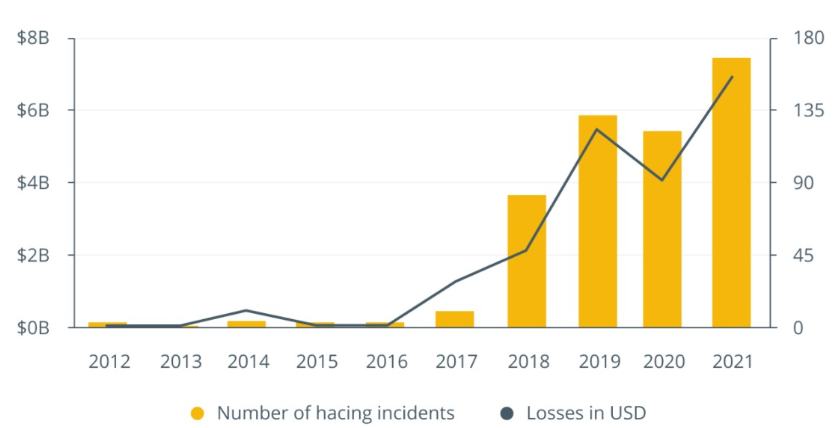
\includegraphics[width=0.8\textwidth]{figures/hack.png}
        % \caption{}
    \end{figure}
    
\end{frame}

%%

\section{Agenda}
\subsection{}
\begin{frame}
    \frametitle{Agenda}

    \begin{itemize}
        \item Backgroud: the importance of contract security
        \item Vulnerabilities in smart contracts
        \begin{itemize}
            \item \textbf{Reentrancy}
            \item Missing Input Validation
            \item Unhandled Exception
            \item Arithmetic Vulnerabilities
            \item Fake EOS
            \item Fake Receipt
            \item Rollback
            \item Missing Permission Check
        \end{itemize}
        \item Vulnerabilities Detection
        \item Automatic Fixes
        \item Evaluation
        \item Reference
    \end{itemize}
    
\end{frame}

%%

\section{Vulnerabilities in smart contracts}
\subsection{}
\begin{frame}
    \frametitle{Reentrancy}

    \begin{itemize}
        \item init
        \begin{itemize}
            \item Attach account: \$100
            \item Employee A
            \item Employee B
        \end{itemize}
        \item attack
        \begin{enumerate}
            \item Request a withdrawal of \$60 from Employee A.
            \item Employee A gives \$60 to the attacker
            \item Request a withdrawal of \$60 from employee B. At this time, employee B does not know that the attacker has already withdrawn \$60 from employee A.
            \item Employee  gives \$60 to the attacker.
            \item Employee B changes the balance of the attacker's bank account. Attacker's account:100 - 60 = 40
            \item Employee A changes the balance of the attacker's bank account. Attacker's account:40 - 60 = -20
        \end{enumerate}
    \end{itemize}

\end{frame}

%%

\section{Vulnerabilities in smart contracts}
\subsection{}
\begin{frame}
    \frametitle{Reentrancy}

    \begin{figure}[h]
        \centering
        \includegraphics[width=0.95\textwidth]{figures/Reentrancy.png}
        \caption{An exploit of Reentrancy vulnerability}
    \end{figure}

    
\end{frame}

%%

\section{Agenda}
\subsection{}
\begin{frame}
    \frametitle{Agenda}

    \begin{itemize}
        \item Backgroud: the importance of contract security
        \item Vulnerabilities in smart contracts
        \begin{itemize}
            \item Reentrancy
            \item Missing Input Validation
            \item Unhandled Exception
            \item Arithmetic Vulnerabilities
            \item Fake EOS
            \item Fake Receipt
            \item Rollback
            \item Missing Permission Check
        \end{itemize}
        \item \textbf{Vulnerabilities Detection}
        \item Automatic Fixes
        \item Evaluation
        \item Reference
    \end{itemize}
    
\end{frame}

%%

\section{Vulnerabilities in smart contracts}
\subsection{}
\begin{frame}
    \frametitle{Vulnerabilities Detection}

    \begin{itemize}
        \item Difference comparison
        \item Find control flow, data flow characteristics
        \item Fuzzing
        \item Using multiple existing tools, and seting thresholds to determine if it is a vulnerability
    \end{itemize}

\end{frame}

%%

\section{Agenda}
\subsection{}
\begin{frame}
    \frametitle{Agenda}

    \begin{itemize}
        \item Backgroud: the importance of contract security
        \item Vulnerabilities in smart contracts
        \begin{itemize}
            \item Reentrancy
            \item Missing Input Validation
            \item Unhandled Exception
            \item Arithmetic Vulnerabilities
            \item Fake EOS
            \item Fake Receipt
            \item Rollback
            \item Missing Permission Check
        \end{itemize}
        \item Vulnerabilities Detection
        \item \textbf{Automatic Fixes}
        \item Evaluation
        \item Reference
    \end{itemize}
    
\end{frame}

%%

\section{Vulnerabilities in smart contracts}
\subsection{}
\begin{frame}
    \frametitle{Automatic Fixes}

    \begin{itemize}
        \item Generates patches using template-based fix patterns and leverages static program analysis
        \item Binary rewriting. Binary rewriting has also been applied to retrofit security hardening techniques such as control-flow integrity, to compiled binaries, but also to dynamically apply security patches to running programs. For binary rewriting on traditional architectures two flavors of approaches have been developed: static and dynamic rewriting.
    \end{itemize}
    
\end{frame}

%%

\section{Agenda}
\subsection{}
\begin{frame}
    \frametitle{Agenda}

    \begin{itemize}
        \item Backgroud: the importance of contract security
        \item Vulnerabilities in smart contracts
        \begin{itemize}
            \item Reentrancy
            \item Missing Input Validation
            \item Unhandled Exception
            \item Arithmetic Vulnerabilities
            \item Fake EOS
            \item Fake Receipt
            \item Rollback
            \item Missing Permission Check
        \end{itemize}
        \item Vulnerabilities Detection
        \item Automatic Fixes
        \item \textbf{Evaluation}
        \item Reference
    \end{itemize}
    
\end{frame}

%%

\section{Vulnerabilities in smart contracts}
\subsection{}
\begin{frame}
    \frametitle{Evaluation}

    \begin{itemize}
        \item False Positives
        \item Runtime Performance
        \item Extra Gas
    \end{itemize}
    
\end{frame}

%%

\section{Agenda}
\subsection{}
\begin{frame}
    \frametitle{Agenda}

    \begin{itemize}
        \item Backgroud: the importance of contract security
        \item Vulnerabilities in smart contracts
        \begin{itemize}
            \item Reentrancy
            \item Missing Input Validation
            \item Unhandled Exception
            \item Arithmetic Vulnerabilities
            \item Fake EOS
            \item Fake Receipt
            \item Rollback
            \item Missing Permission Check
        \end{itemize}
        \item Vulnerabilities Detection
        \item Automatic Fixes
        \item Evaluation
        \item \textbf{Reference}
    \end{itemize}
    
\end{frame}

%%

\section{Reference}
\subsection{}
\begin{frame}
    \frametitle{Reference}
    
    \begin{quotation}
        [1] Q. Le, “How hackers attack eos contracts and ways to prevent it,” nov 2018.

        [2] N. He, R. Zhang, H. Wang, L. Wu, X. Luo, Y. Guo, T. Yu, and X. Jiang, “EOSAFE: Security analysis of EOSIO smart contracts,” in 30th USENIX Security Symposium (USENIX Security 21), USENIX Association, aug 2021.

        [3] D. Wang, B. Jiang, and W. K. Chan, “Wana: Symbolic ex- ecution of wasm bytecode for cross-platform smart contract vulnerability detection,” ArXiv, vol. abs/2007.15510, 2020.

        [4] “Eosio developer portal.”

        [5] “Webassembly 1.0 has shipped in 4 major browser engines..” 
    \end{quotation}

\end{frame}

%%

\section{Reference}
\subsection{}
\begin{frame}
    \frametitle{Reference}
    
    \begin{quotation}
        [6] ““transactions protocol,”.”

        [7] “”fake eos attack” upgraded, 60k eos tokens lost by eoscast.”
        [8] “Roll back attack about blacklist in eos.”

        [9] ““dappradar, a dapp browser,”,” dct 2020.

        [10] “Dapptotal„” nov 2019.

        [11] ““blogs about blockchain security events,”,” 2020. 

        [12] ““blockchain security events,”.”
    \end{quotation}

\end{frame}

\end{document}